
\definecolor{tableheader}{rgb}{0.8, 0.8, 0.8}
\definecolor{tableevenrow}{rgb}{0.95, 0.95, 0.95}
\definecolor{tableoddrow}{rgb}{1.0, 1.0, 1.0}

%----------------------------------------------------------------------------------------
\chapter{Contesto lavorativo}
\label{cap:introduzione}
\section{Profilo aziendale}
Zero12 s.r.l. è una \textit{startup} italiana fondata nel 2012 con attualmente due sedi operative, la prima a Padova (dove ho svolto il periodo di \textit{stage}) e la seconda ad Empoli. 
L'azienda è \textit{partner} \gls{awsg} ed è specializzata nella realizzazione di applicazioni \textit{cloud native} e dello sviluppo di applicazioni e servizi \textit{web} e \textit{mobile}, offrendo ai propri clienti, proveniente da ambiti diversificati, soluzioni flessibili e scalibili.\\
Il team di Zero12 s.r.l. non si limita alla realizzazione di applicazioni, ma si estende alla creazione di un percorso di innovazione condiviso con i clienti. Questo percorso mira a integrare nelle realtà aziendali le tecnologie più adatte alle specifiche esigenze, assicurando un miglioramento continuo dei processi aziendali e un’efficace presenza sul web.\\
L'azienda è parte di Var Group s.p.a, un' azienda italiana che supporta i propri \textit{partner} con servizi e competenze per raggiungere gli obiettivi prefissati.
\section{Organizzazione aziendale}
Durante il mio periodo di \textit{stage} ho avuto modo osservare in prima persona l'organizzazione in \textit{team} di lavoro che l'azienda adotta.
I ruoli che ho potuto osservare sono rappresentati di seguito nella tabella \ref{tab:ruoli}.
\begin{longtable}{|>{\RaggedRight\arraybackslash}p{3.5cm}|>{\RaggedRight\arraybackslash}p{8.5cm}|}
    \hline
    \rowcolor{tableheader}\textbf{Ruolo} & \textbf{Descrizione} \\
    \hline
    \endfirsthead

    \rowcolor{tableheader}\textbf{Ruolo} & \textbf{Descrizione} \\
    \hline
    \endhead

    \hline
    \endfoot

    \hline
    \endlastfoot

    \rowcolor{tableoddrow}\textbf{\textit{CEO}} & Il \gls{ceog} rappresenta il ruolo più alto all'interno dell'azienda. È responsabile di definire la strategia e le decisioni più importanti dell'azienda. Supervisiona i processi aziendali e gestisce i contatti con potenziali nuovi clienti. \\
    \hline
    \rowcolor{tableevenrow}\textbf{\textit{Project manager}} & Il \textit{project manager} è la figura che si occupa di coordinare il proprio team di lavoro, gestendo le risorse e le tempistiche di progetto e interfacciandosi con il cliente. Il mio \textit{tutor} aziendale, svolge anche il ruolo di \textit{project manager} e ho avuto modo di osservare il suo lavoro in prima persona.\\
    \hline
    \rowcolor{tableoddrow}\textbf{\textit{Software developer}} & Il \textit{software developer} è la figura che si occupa della progettazione e dello sviluppo delle varie componenti \textit{software} individuate durante la fase di analisi e progettazione. Ognuno di loro si specializza nello sviluppo di funzionalità di \textit{frontend}, \textit{backend} o entrambi (\textit{fullstack}) a seconda delle competenze e delle preferenze personali.
    Durante il mio periodo di \textit{stage} ho assunto questo ruolo.\\
    \hline
    \rowcolor{tableevenrow}\textbf{\textit{Mobile developer}} & Il \textit{mobile developer} è la figura che si occupa della stessa mansione del \textit{software developer} per un'applicazione \textit{mobile}. All'interno dell'azienda Zero12 s.r.l. i \textit{mobile developers} si suddividono in due categorie: \textit{Android developers} e \textit{iOS developers}.\\
    \hline
    \rowcolor{tableoddrow}\textbf{\textit{AWS specialist}} & L'\textit{AWS Specialist} è la figura specializzata nella configurazione, gestione e adozione dei servizi offerti da \gls{aws}.\\
    \hline
    \rowcolor{tableevenrow}\textbf{\textit{HR}} & La figura dell' \gls{hrg} è una figura che si occupa della gestione delle risorse umane all'interno dell'azienda.\\
    \hline
    \caption{Organizzazione dei ruoli all'interno di Zero12 s.r.l.}
    \label{tab:ruoli}
\end{longtable}
Ad ogni nuovo progetto viene assegnato un \textit{team} di lavoro composto da un \textit{project manager}, un numero variabile di \textit{software developers} o \textit{mobile developers}, a seconda delle esigenze del progetto, e un \textit{AWS specialist} se il progetto prevede l'utilizzo di servizi \gls{aws}. 
\pagebreak
\section{Processi e tecnologie}
\subsection{Metodologia di sviluppo}
Durante il mio periodo di \textit{stage} ho avuto modo di sperimentare in prima persona i processi istanziati dall'azienda per la realizzazione di un progetto.
La metodologia di lavoro adottata è quella \textit{Agile} e in particolare il \textit{framework Scrum}.\\ 
Il \textit{framework Scrum} prevede la suddivisione del progetto in \textit{Sprint} di durata fissa (durante il mio periodo di \textit{stage} la durata era di una settimana) e la definizione di un \textit{team} di lavoro (il \textit{team} di lavoro era composto dal mio \textit{tutor} aziendale come \textit{project manager} e da me come \textit{software developer}).
\begin{figure}[H]
    \centering
    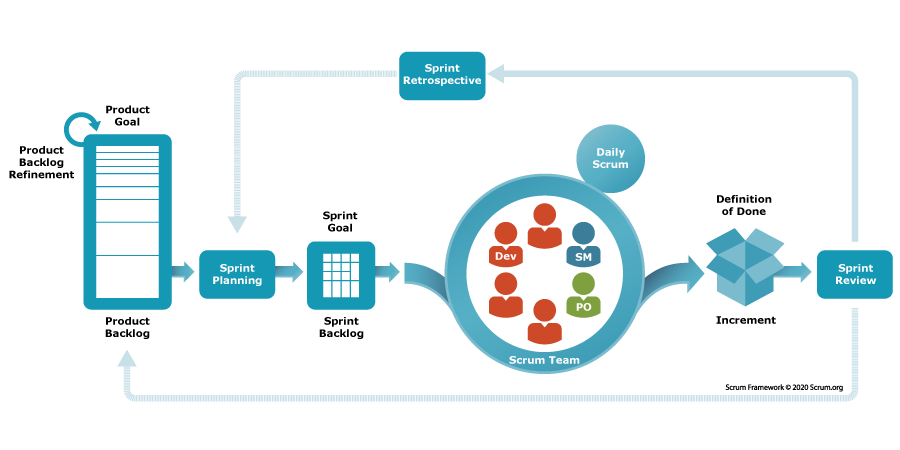
\includegraphics[width=0.9\textwidth]{scrum.png}
    \caption{Schema di flusso di un progetto con metodologia \textit{Scrum}}
    \small \textbf{Fonte:} \url{www.scrum.org}
    \label{fig:scrum}
\end{figure}
Nella figura \ref{fig:scrum} viene mostrato il flusso di lavoro di un progetto con metodologia \textit{Scrum}. All'interno dell'azienda, il flusso di lavoro segue il seguente schema:
\begin{itemize}
    \item \textit{\gls{User-stories}}: all'inizio viene effettuata una prima sessione di \textit{user stories mapping} che va a definire quello che sarà presente nel \textit{product backlog}. Questa sessione viene svolta insieme al cliente, in modo da avere una chiara visione delle aspettative del cliente, definendo cosi anche le \textit{feature} più importanti da sviluppare.
    \item \textbf{\textit{Sprint planning}}: all'inizio di ogni \textit{sprint} vengono selezionate le \textit{task} da svolgere, in base alla priorità, dal \textit{product backlog} e vengono assegnate ai membri del \textit{team} di lavoro.
    \item \textbf{\textit{Sprint review}}: alla fine di ogni \textit{sprint} viene effettuata una revisione del lavoro svolto, andando a controllare che le \textit{task} assegnate siano state completate e che il lavoro svolto sia stato svolto in modo conforme alle aspettative del cliente.
    \item \textbf{\textit{Sprint retrospective}}: alla fine di ogni \textit{sprint} viene effettuato un controllo interno del lavoro svolto durante lo \textit{sprint}, andando ad evidenziare eventuali problematiche sorte e andando a definire eventuali miglioramenti da apportare al processo di lavoro.
\end{itemize}
\subsection{Strumenti di supporto ai processi}
\subsubsection{Jira}
\textit{Jira} è un \gls{itsg} sviluppato da \textit{Atlassian} che permette la gestione dei progetti in modo \textit{Agile}. Inoltre permette la gestione di \textit{ticket} e la creazione di \textit{board} personalizzate per la gestione dei progetti.
All'inizio di ogni \textit{sprint}, lo \textit{scrum master} crea una nuova \textit{board} relativa allo \textit{sprint} in corso e assegna le \textit{task} da svolgere ai membri del \textit{team} di lavoro.
I membri del \textit{team} di lavoro posso spostare i \textit{ticket} da una colonna all'altra: 
\begin{itemize}
    \item \textbf{Da completare}: \textit{Ticket} assegnati ma che devono essere ancora completati.
    \item \textbf{In corso}: \textit{Ticket} assegnati ad una o più risorse del \textit{team} di lavoro e che sono in fase di sviluppo.
    \item \textbf{Completato}; \textit{Ticket} completati e pronti per la revisione.
\end{itemize}
\begin{figure}[H]
    \centering
    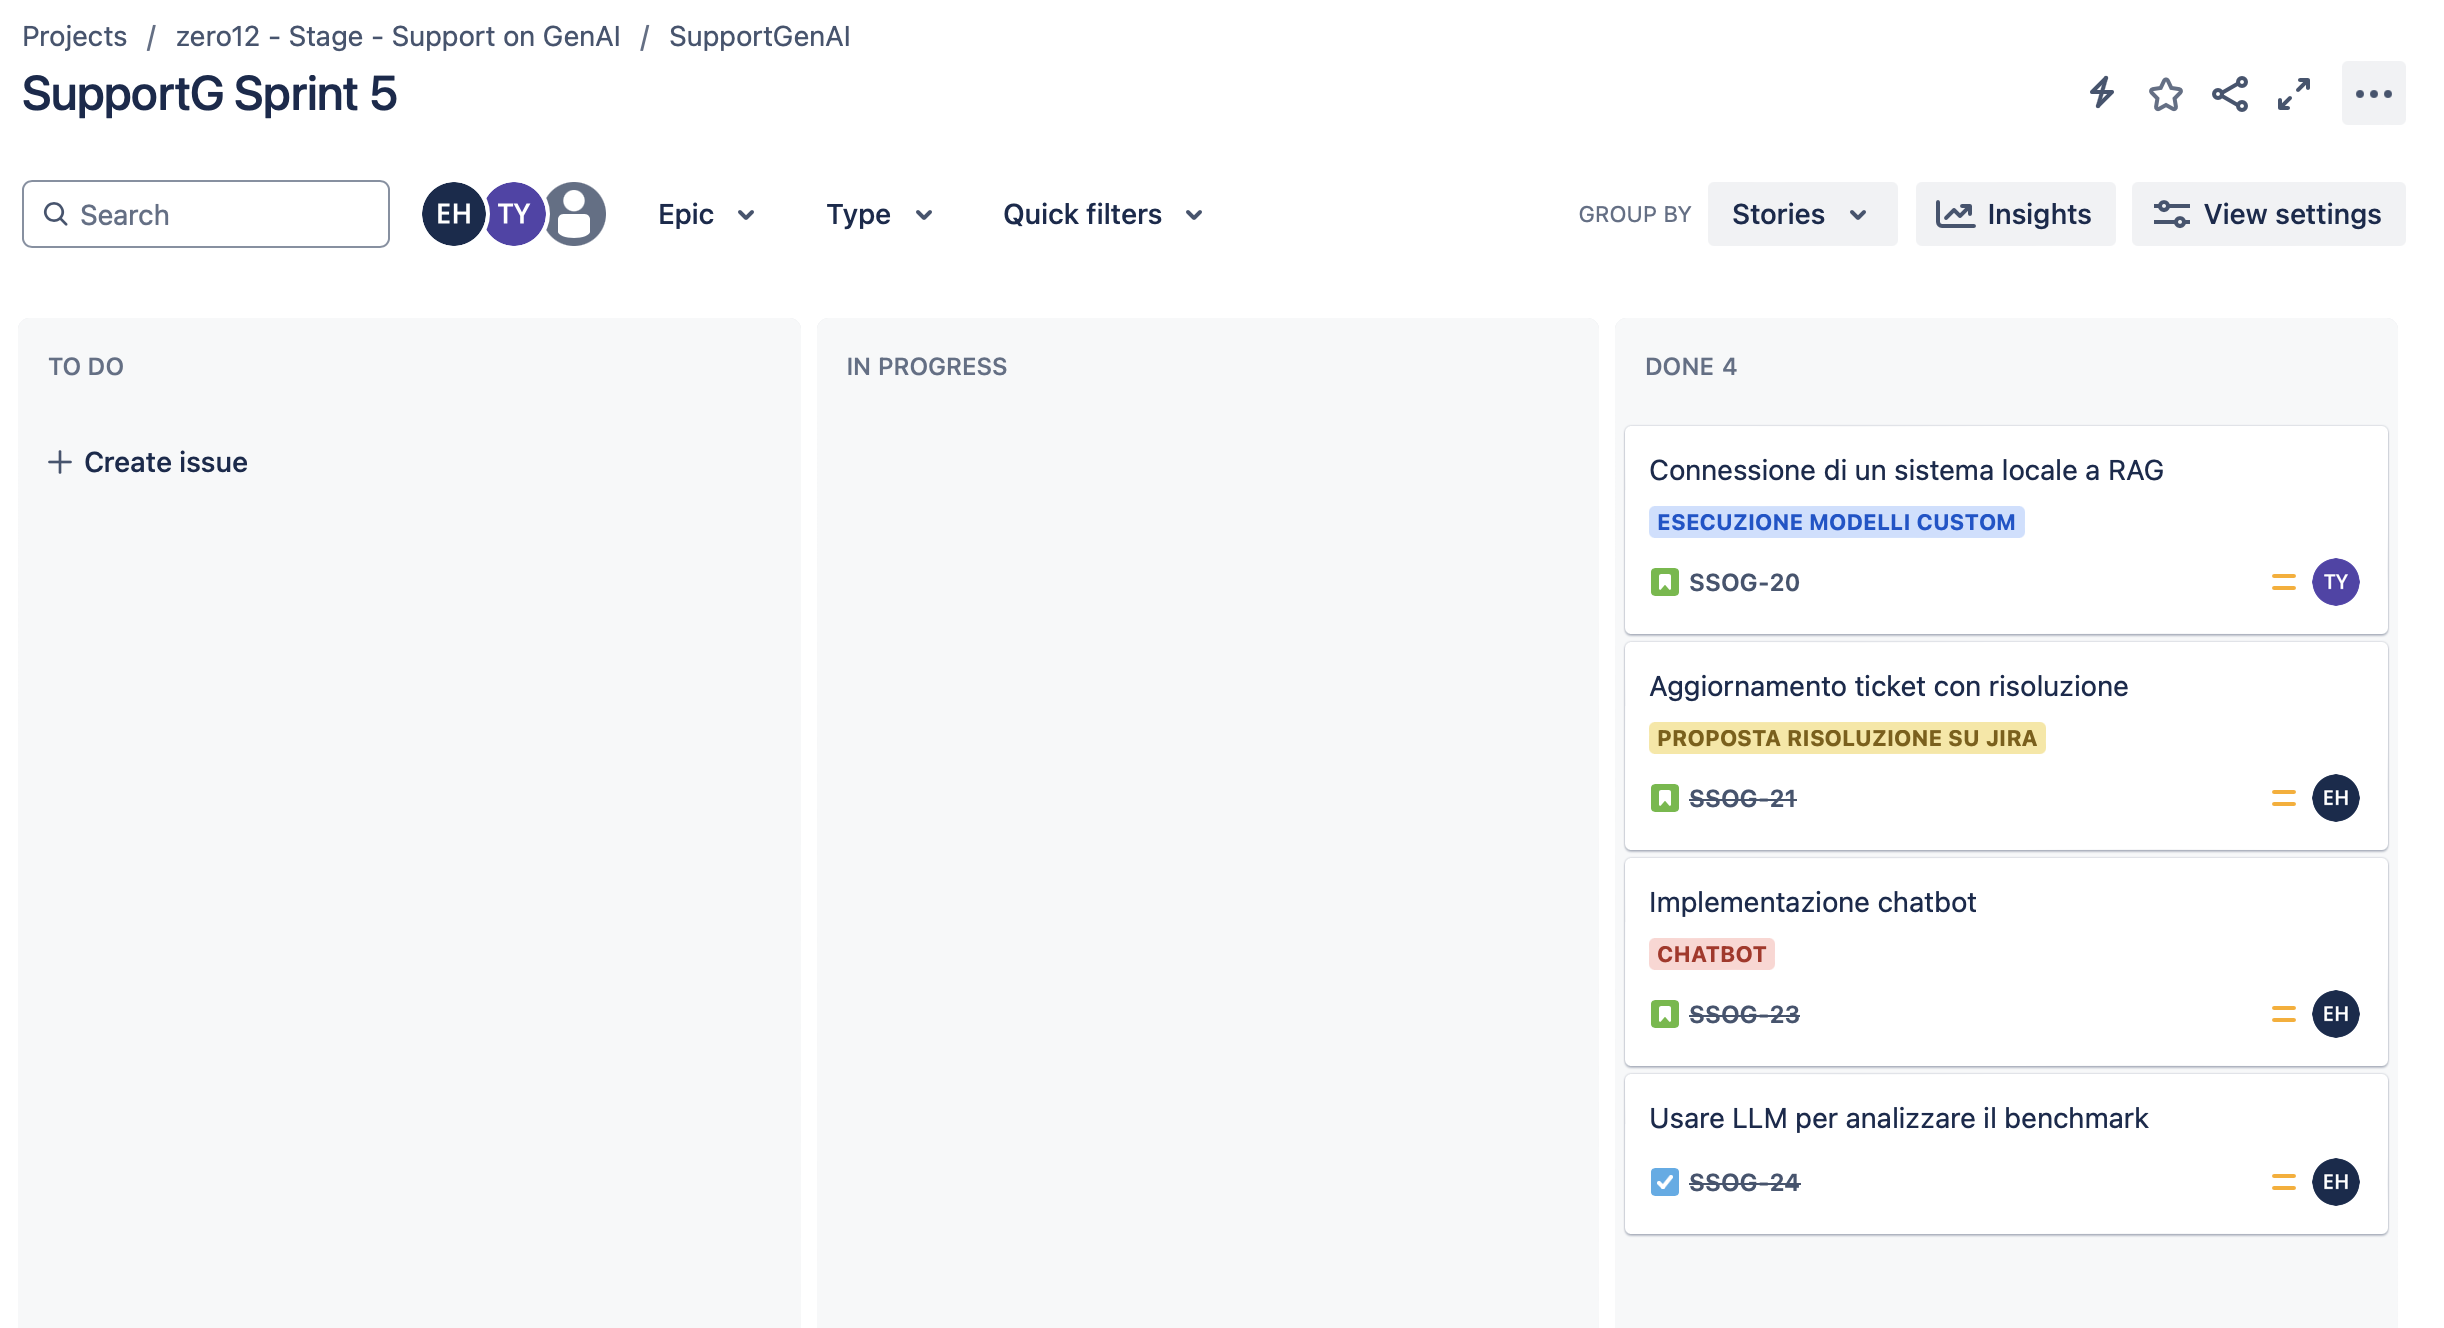
\includegraphics[width=0.9\textwidth]{Jira.png}
    \caption{\textit{Board} del quinto \textit{sprint} del progetto di \textit{stage}}
    \label{fig:Jira}
\end{figure}

\subsubsection{\textit{Visual Studio Code}}
\textit{Visual Studio Code} è un \textit{editor} di codice sorgente sviluppato da \textit{Microsoft} che permette la scrittura di codice in diversi linguaggi di programmazione.

\subsubsection{Github}
\textit{Github} è una piattaforma \textit{web} che permette il versionamento del codice sorgente tramite il sistema di controllo di versione \textit{Git}. 
Grazie a questo strumento, è possibile creare \textit{repositories} in cui salvare il codice sorgente del progetto. 
È possibile suddividere il progetto in \textit{branch} ed assegnare ad ogni \textit{branch} una \textit{task} da svolgere. Una volta completata la \textit{task}, il \textit{branch} viene unito al \textit{branch} principale tramite una \textit{pull request}. 
Tramite questa pratica è possibile revisionare il codice sorgente prodotto e garantire che il codice prodotto sia conforme alla qualità richiesta.
\begin{figure}[H]
    \centering
    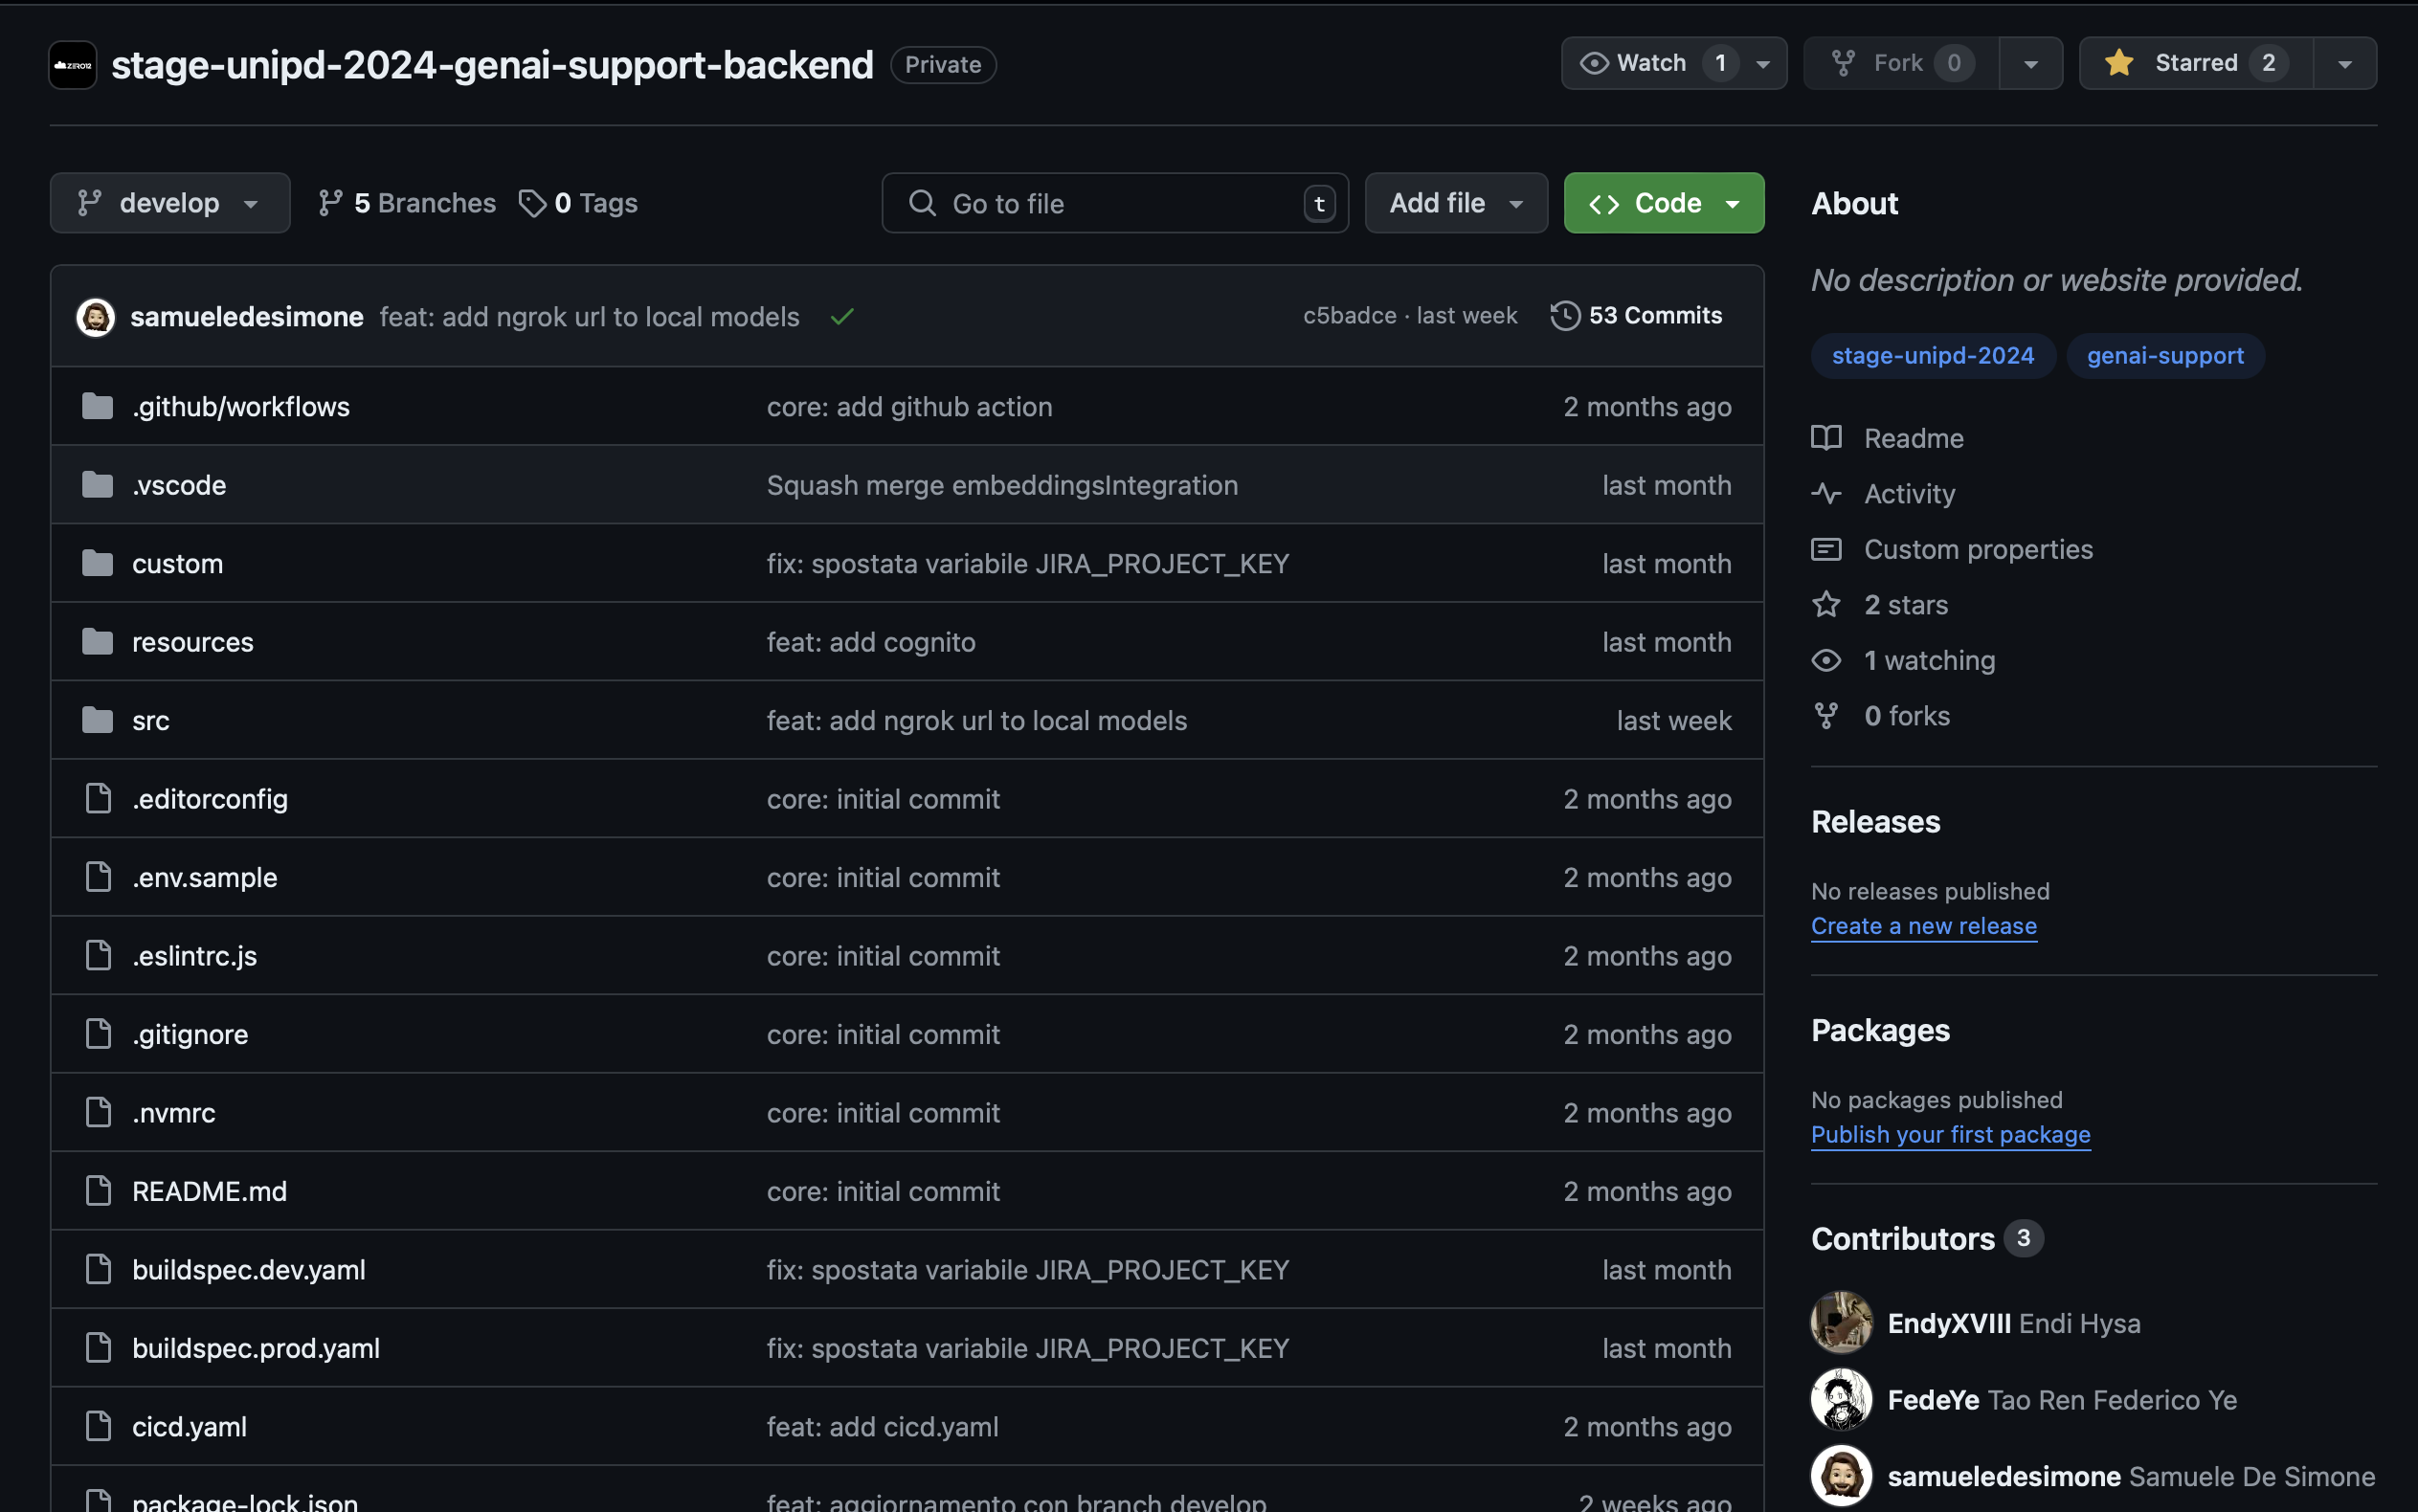
\includegraphics[width=0.9\textwidth]{github.png}
    \caption{Schermata del \textit{repository} Github del progetto di \textit{stage}}
    \label{fig:Github}
\end{figure}
\subsubsection{\gls{slackg}}
\gls{slackg} è una piattaforma di messaggistica istantanea utilizzata nell'ambito lavorativo per la comunicazione interna tra i membri del \textit{team}.
Si possono creare canali di comunicazione dedicati a specifici argomenti. In ambito aziendale, viene creato un canale dedicato ad ogni progetto in modo da poter permettere una comunicazione più efficace tra i membri del \textit{team} di lavoro.
Nel caso del mio progetto di \textit{stage} è stato creato un canale dedicato al progetto assieme al mio \textit{tutor} aziendale ed un altra figura per aiutarmi in caso di problematiche.
\begin{figure}[H]
    \centering
    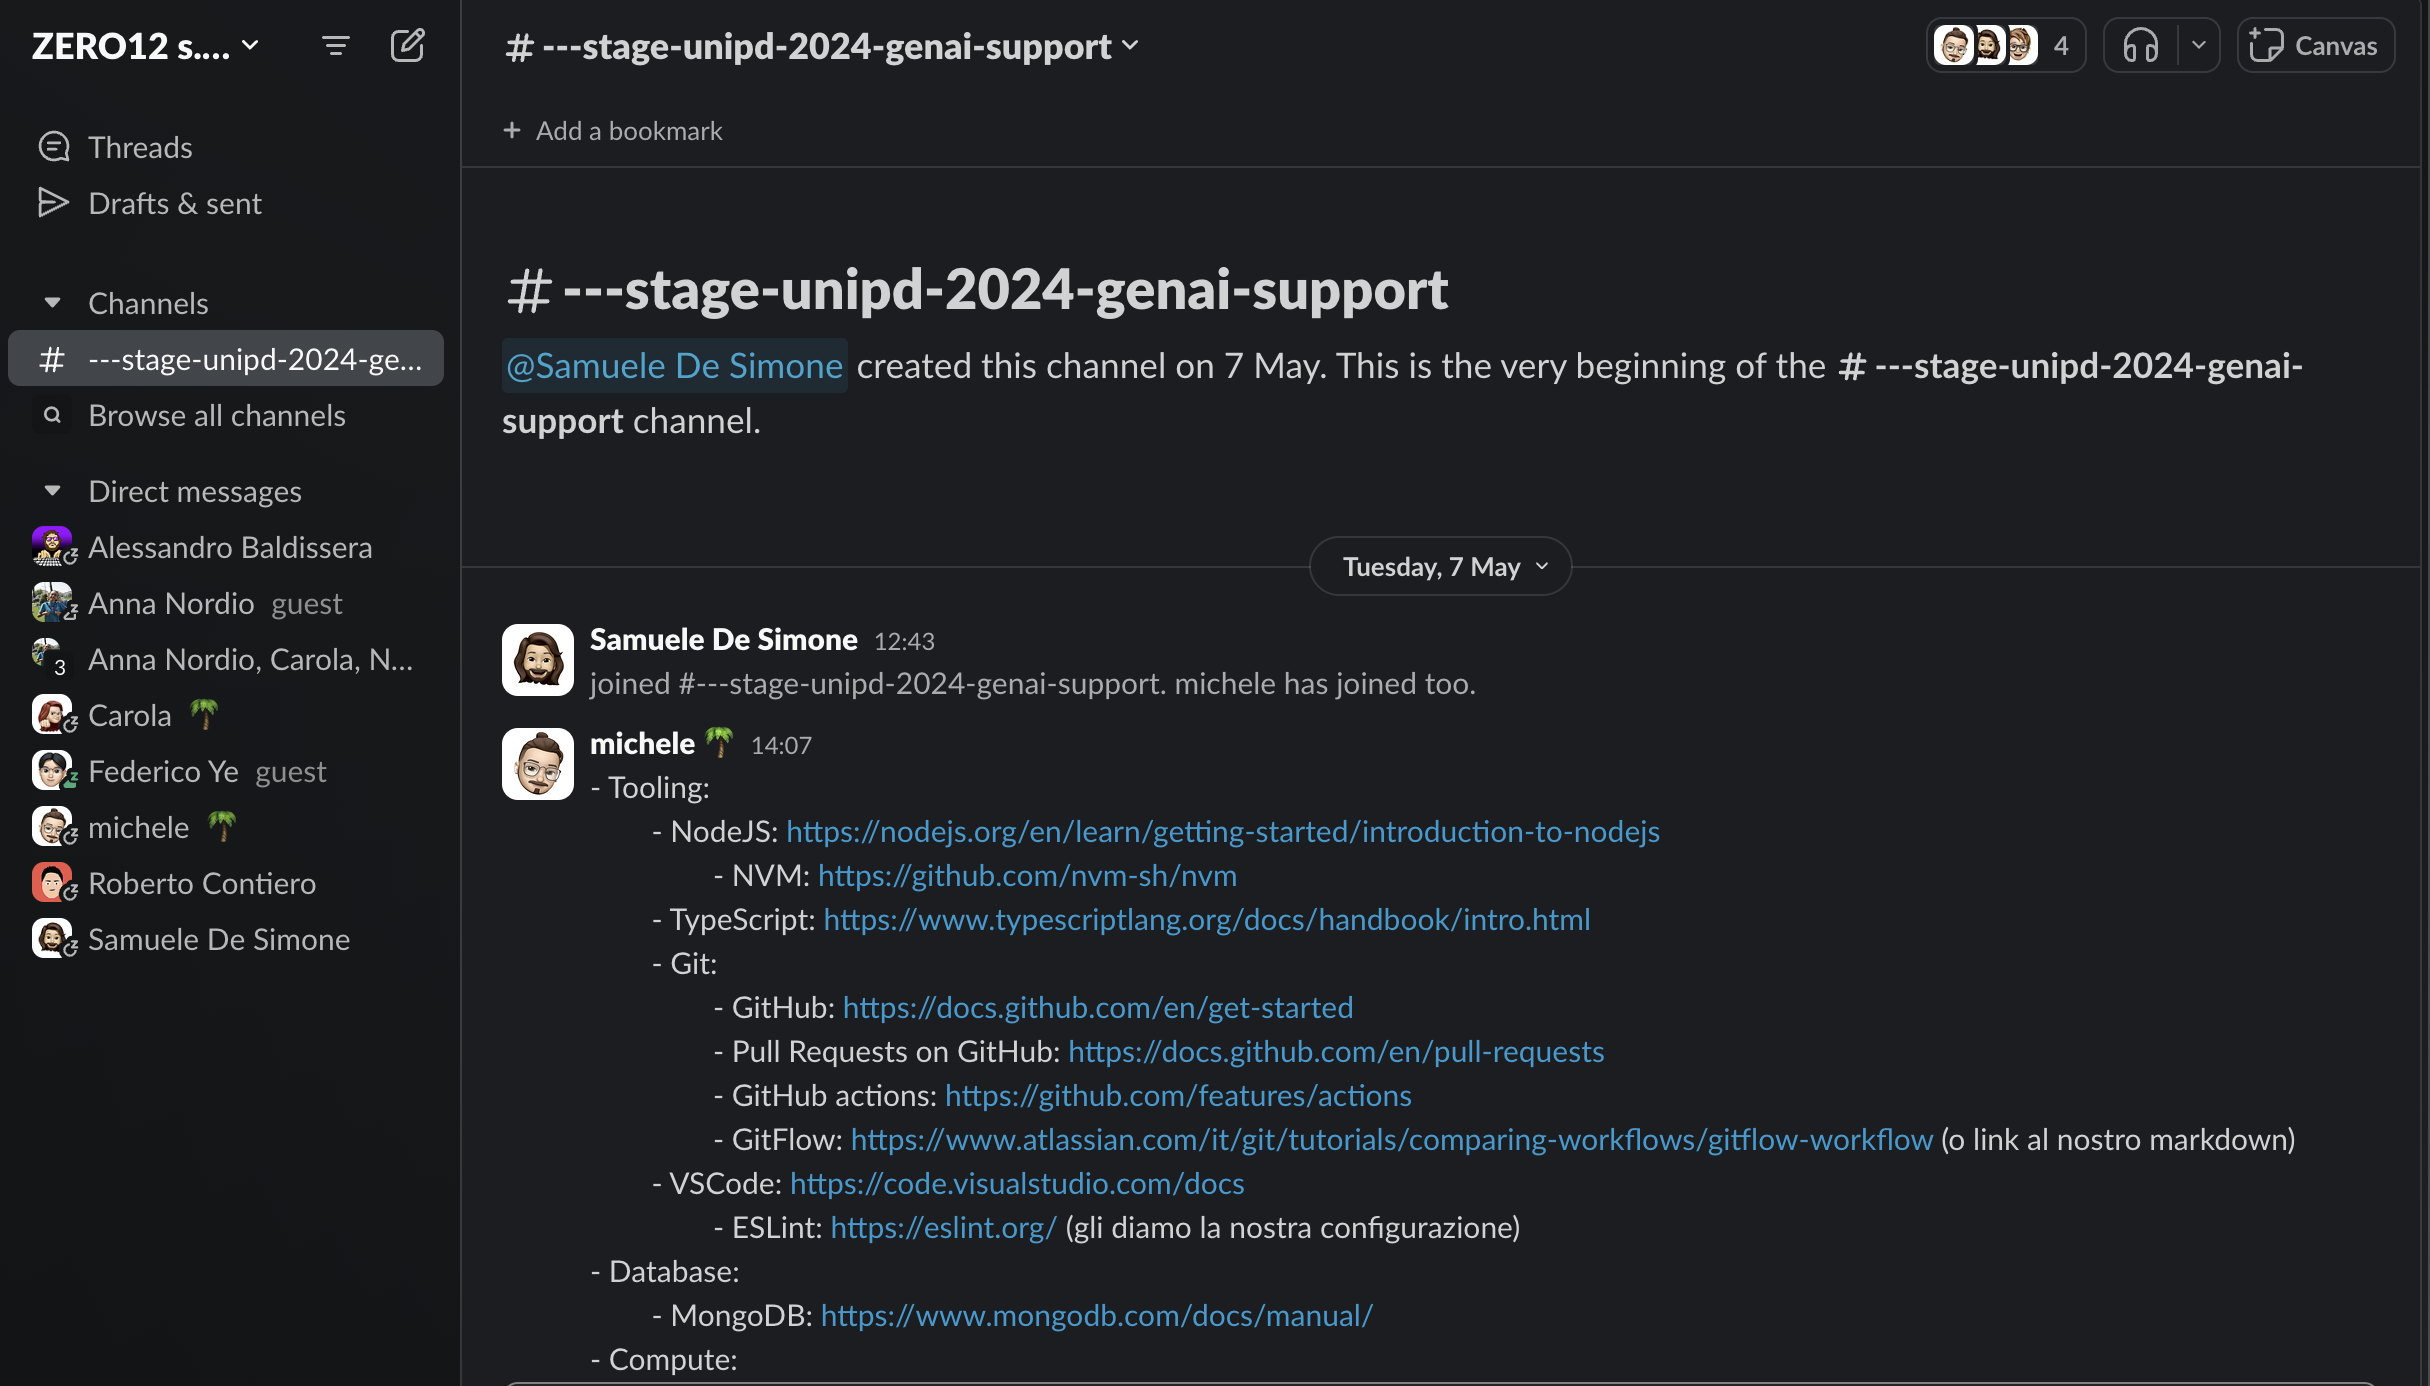
\includegraphics[width=0.9\textwidth]{slack.png}
    \caption{Schermata del canale dedicato al progetto di \textit{stage}}
    \label{fig:Slack}
\end{figure}
\subsection{Tecnologie utilizzate}
\subsubsection{Typescript}
Typescript è un linguaggio di programmazione sviluppato da \textit{Microsoft} che estende il linguaggio \textit{Javascript} aggiungendo la possibilità di definire tipi alle variabili.
Questa estensione permette di rendere retrocompatibile il codice scritto in \texit{Javascript} con il codice scritto in \textit{Typescript} e di ridurre il numero di errori di programmazione.


%\noindent Esempio di utilizzo di un termine nel glossario \\
%\gls{api}. \\

%\noindent Esempio di citazione in linea \\
%\cite{site:Agile-manifesto}. \\

%\noindent Esempio di citazione nel pie' di pagina \\
%citazione\footcite{womak:lean-thinking} \\

\section{Tipologia di clientela}
Analisi della tipologia di clientela dell'azienda.

\section{Propensione all'innovazione}
Valutazione dell'approccio dell'azienda verso l'innovazione e nuove tecnologie

%\section{Organizzazione del testo}

%\begin{description}
    %\item[{\hyperref[cap:introduzione]{Il primo capitolo}}] descrive ...
    %\item[{\hyperref[cap:lo-stage]{Il secondo capitolo}}] descrive ...
    
    %\item[{\hyperref[cap:descrizione-stage]{Il terzo capitolo}}] approfondisce ...
    
    %\item[{\hyperref[cap:conclusioni]{Il quarto capitolo}}] approfondisce ...
    
%\end{description}

%Riguardo la stesura del testo, relativamente al documento sono state adottate le seguenti convenzioni tipografiche:
%\begin{itemize}
	%\item gli acronimi, le abbreviazioni e i termini ambigui o di uso non comune menzionati vengono definiti nel glossario, situato alla fine del presente documento;
	%\item per la prima occorrenza dei termini riportati nel glossario viene utilizzata la seguente nomenclatura: \emph{parola}\glsfirstoccur;
	%\item i termini in lingua straniera o facenti parti del gergo tecnico sono evidenziati con il carattere \emph{corsivo}.
%\end{itemize}
